% Created by tikzDevice version 0.12.3.1 on 2023-03-15 09:24:51
% !TEX encoding = UTF-8 Unicode
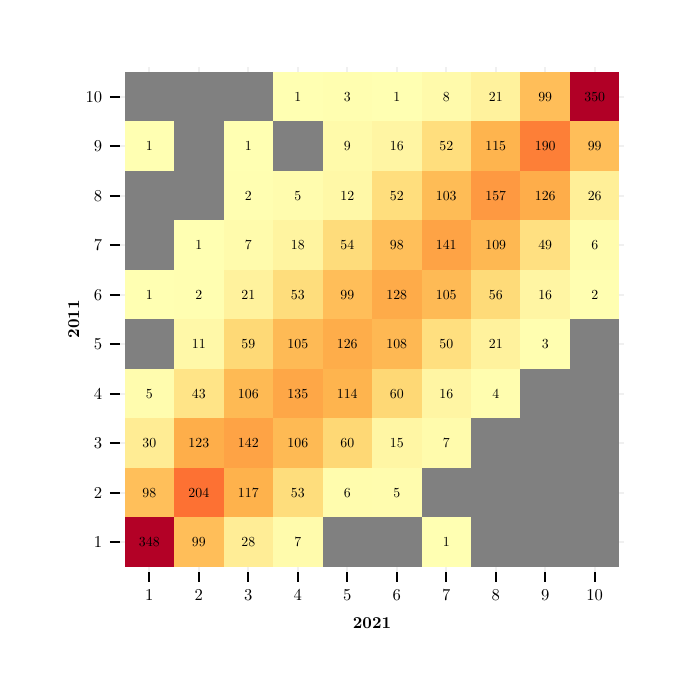
\begin{tikzpicture}[x=1pt,y=1pt]
\definecolor{fillColor}{RGB}{255,255,255}
\path[use as bounding box,fill=fillColor,fill opacity=0.00] (0,0) rectangle (231.26,231.26);
\begin{scope}
\path[clip] (  1.40,  0.00) rectangle (229.86,231.26);
\definecolor{fillColor}{RGB}{255,255,255}

\path[fill=fillColor] (  1.40,  0.00) rectangle (229.86,231.26);
\end{scope}
\begin{scope}
\path[clip] ( 33.23, 34.63) rectangle (215.64,217.04);
\definecolor{fillColor}{RGB}{255,255,255}

\path[fill=fillColor] ( 33.23, 34.63) rectangle (215.64,217.04);
\definecolor{drawColor}{gray}{0.94}

\path[draw=drawColor,line width= 0.7pt,line join=round] ( 33.23, 45.36) --
	(215.64, 45.36);

\path[draw=drawColor,line width= 0.7pt,line join=round] ( 33.23, 63.24) --
	(215.64, 63.24);

\path[draw=drawColor,line width= 0.7pt,line join=round] ( 33.23, 81.13) --
	(215.64, 81.13);

\path[draw=drawColor,line width= 0.7pt,line join=round] ( 33.23, 99.01) --
	(215.64, 99.01);

\path[draw=drawColor,line width= 0.7pt,line join=round] ( 33.23,116.89) --
	(215.64,116.89);

\path[draw=drawColor,line width= 0.7pt,line join=round] ( 33.23,134.78) --
	(215.64,134.78);

\path[draw=drawColor,line width= 0.7pt,line join=round] ( 33.23,152.66) --
	(215.64,152.66);

\path[draw=drawColor,line width= 0.7pt,line join=round] ( 33.23,170.54) --
	(215.64,170.54);

\path[draw=drawColor,line width= 0.7pt,line join=round] ( 33.23,188.43) --
	(215.64,188.43);

\path[draw=drawColor,line width= 0.7pt,line join=round] ( 33.23,206.31) --
	(215.64,206.31);

\path[draw=drawColor,line width= 0.7pt,line join=round] ( 43.96, 34.63) --
	( 43.96,217.04);

\path[draw=drawColor,line width= 0.7pt,line join=round] ( 61.84, 34.63) --
	( 61.84,217.04);

\path[draw=drawColor,line width= 0.7pt,line join=round] ( 79.73, 34.63) --
	( 79.73,217.04);

\path[draw=drawColor,line width= 0.7pt,line join=round] ( 97.61, 34.63) --
	( 97.61,217.04);

\path[draw=drawColor,line width= 0.7pt,line join=round] (115.49, 34.63) --
	(115.49,217.04);

\path[draw=drawColor,line width= 0.7pt,line join=round] (133.38, 34.63) --
	(133.38,217.04);

\path[draw=drawColor,line width= 0.7pt,line join=round] (151.26, 34.63) --
	(151.26,217.04);

\path[draw=drawColor,line width= 0.7pt,line join=round] (169.14, 34.63) --
	(169.14,217.04);

\path[draw=drawColor,line width= 0.7pt,line join=round] (187.02, 34.63) --
	(187.02,217.04);

\path[draw=drawColor,line width= 0.7pt,line join=round] (204.91, 34.63) --
	(204.91,217.04);
\definecolor{fillColor}{RGB}{179,1,38}

\path[fill=fillColor] ( 35.02, 36.42) rectangle ( 52.90, 54.30);
\definecolor{fillColor}{RGB}{255,191,90}

\path[fill=fillColor] ( 35.02, 54.30) rectangle ( 52.90, 72.19);
\definecolor{fillColor}{RGB}{255,236,148}

\path[fill=fillColor] ( 35.02, 72.19) rectangle ( 52.90, 90.07);
\definecolor{fillColor}{RGB}{255,252,174}

\path[fill=fillColor] ( 35.02, 90.07) rectangle ( 52.90,107.95);
\definecolor{fillColor}{gray}{0.50}

\path[fill=fillColor] ( 35.02,107.95) rectangle ( 52.90,125.83);
\definecolor{fillColor}{RGB}{255,255,178}

\path[fill=fillColor] ( 35.02,125.83) rectangle ( 52.90,143.72);
\definecolor{fillColor}{gray}{0.50}

\path[fill=fillColor] ( 35.02,143.72) rectangle ( 52.90,161.60);

\path[fill=fillColor] ( 35.02,161.60) rectangle ( 52.90,179.48);
\definecolor{fillColor}{RGB}{255,255,178}

\path[fill=fillColor] ( 35.02,179.48) rectangle ( 52.90,197.37);
\definecolor{fillColor}{gray}{0.50}

\path[fill=fillColor] ( 35.02,197.37) rectangle ( 52.90,215.25);
\definecolor{fillColor}{RGB}{255,190,89}

\path[fill=fillColor] ( 52.90, 36.42) rectangle ( 70.79, 54.30);
\definecolor{fillColor}{RGB}{253,113,51}

\path[fill=fillColor] ( 52.90, 54.30) rectangle ( 70.79, 72.19);
\definecolor{fillColor}{RGB}{254,174,74}

\path[fill=fillColor] ( 52.90, 72.19) rectangle ( 70.79, 90.07);
\definecolor{fillColor}{RGB}{255,228,135}

\path[fill=fillColor] ( 52.90, 90.07) rectangle ( 70.79,107.95);
\definecolor{fillColor}{RGB}{255,248,168}

\path[fill=fillColor] ( 52.90,107.95) rectangle ( 70.79,125.83);
\definecolor{fillColor}{RGB}{255,254,177}

\path[fill=fillColor] ( 52.90,125.83) rectangle ( 70.79,143.72);
\definecolor{fillColor}{RGB}{255,255,178}

\path[fill=fillColor] ( 52.90,143.72) rectangle ( 70.79,161.60);
\definecolor{fillColor}{gray}{0.50}

\path[fill=fillColor] ( 52.90,161.60) rectangle ( 70.79,179.48);

\path[fill=fillColor] ( 52.90,179.48) rectangle ( 70.79,197.37);

\path[fill=fillColor] ( 52.90,197.37) rectangle ( 70.79,215.25);
\definecolor{fillColor}{RGB}{255,237,150}

\path[fill=fillColor] ( 70.79, 36.42) rectangle ( 88.67, 54.30);
\definecolor{fillColor}{RGB}{254,178,76}

\path[fill=fillColor] ( 70.79, 54.30) rectangle ( 88.67, 72.19);
\definecolor{fillColor}{RGB}{254,163,69}

\path[fill=fillColor] ( 70.79, 72.19) rectangle ( 88.67, 90.07);
\definecolor{fillColor}{RGB}{254,186,84}

\path[fill=fillColor] ( 70.79, 90.07) rectangle ( 88.67,107.95);
\definecolor{fillColor}{RGB}{254,217,118}

\path[fill=fillColor] ( 70.79,107.95) rectangle ( 88.67,125.83);
\definecolor{fillColor}{RGB}{255,242,157}

\path[fill=fillColor] ( 70.79,125.83) rectangle ( 88.67,143.72);
\definecolor{fillColor}{RGB}{255,251,172}

\path[fill=fillColor] ( 70.79,143.72) rectangle ( 88.67,161.60);
\definecolor{fillColor}{RGB}{255,254,177}

\path[fill=fillColor] ( 70.79,161.60) rectangle ( 88.67,179.48);
\definecolor{fillColor}{RGB}{255,255,178}

\path[fill=fillColor] ( 70.79,179.48) rectangle ( 88.67,197.37);
\definecolor{fillColor}{gray}{0.50}

\path[fill=fillColor] ( 70.79,197.37) rectangle ( 88.67,215.25);
\definecolor{fillColor}{RGB}{255,251,172}

\path[fill=fillColor] ( 88.67, 36.42) rectangle (106.55, 54.30);
\definecolor{fillColor}{RGB}{254,221,124}

\path[fill=fillColor] ( 88.67, 54.30) rectangle (106.55, 72.19);
\definecolor{fillColor}{RGB}{254,186,84}

\path[fill=fillColor] ( 88.67, 72.19) rectangle (106.55, 90.07);
\definecolor{fillColor}{RGB}{254,167,71}

\path[fill=fillColor] ( 88.67, 90.07) rectangle (106.55,107.95);
\definecolor{fillColor}{RGB}{254,186,85}

\path[fill=fillColor] ( 88.67,107.95) rectangle (106.55,125.83);
\definecolor{fillColor}{RGB}{254,221,124}

\path[fill=fillColor] ( 88.67,125.83) rectangle (106.55,143.72);
\definecolor{fillColor}{RGB}{255,244,160}

\path[fill=fillColor] ( 88.67,143.72) rectangle (106.55,161.60);
\definecolor{fillColor}{RGB}{255,252,174}

\path[fill=fillColor] ( 88.67,161.60) rectangle (106.55,179.48);
\definecolor{fillColor}{gray}{0.50}

\path[fill=fillColor] ( 88.67,179.48) rectangle (106.55,197.37);
\definecolor{fillColor}{RGB}{255,255,178}

\path[fill=fillColor] ( 88.67,197.37) rectangle (106.55,215.25);
\definecolor{fillColor}{gray}{0.50}

\path[fill=fillColor] (106.55, 36.42) rectangle (124.43, 54.30);
\definecolor{fillColor}{RGB}{255,252,173}

\path[fill=fillColor] (106.55, 54.30) rectangle (124.43, 72.19);
\definecolor{fillColor}{RGB}{254,216,117}

\path[fill=fillColor] (106.55, 72.19) rectangle (124.43, 90.07);
\definecolor{fillColor}{RGB}{254,180,78}

\path[fill=fillColor] (106.55, 90.07) rectangle (124.43,107.95);
\definecolor{fillColor}{RGB}{254,173,74}

\path[fill=fillColor] (106.55,107.95) rectangle (124.43,125.83);
\definecolor{fillColor}{RGB}{255,190,89}

\path[fill=fillColor] (106.55,125.83) rectangle (124.43,143.72);
\definecolor{fillColor}{RGB}{254,220,123}

\path[fill=fillColor] (106.55,143.72) rectangle (124.43,161.60);
\definecolor{fillColor}{RGB}{255,248,167}

\path[fill=fillColor] (106.55,161.60) rectangle (124.43,179.48);
\definecolor{fillColor}{RGB}{255,250,170}

\path[fill=fillColor] (106.55,179.48) rectangle (124.43,197.37);
\definecolor{fillColor}{RGB}{255,254,176}

\path[fill=fillColor] (106.55,197.37) rectangle (124.43,215.25);
\definecolor{fillColor}{gray}{0.50}

\path[fill=fillColor] (124.43, 36.42) rectangle (142.32, 54.30);
\definecolor{fillColor}{RGB}{255,252,174}

\path[fill=fillColor] (124.43, 54.30) rectangle (142.32, 72.19);
\definecolor{fillColor}{RGB}{255,246,164}

\path[fill=fillColor] (124.43, 72.19) rectangle (142.32, 90.07);
\definecolor{fillColor}{RGB}{254,216,117}

\path[fill=fillColor] (124.43, 90.07) rectangle (142.32,107.95);
\definecolor{fillColor}{RGB}{254,184,83}

\path[fill=fillColor] (124.43,107.95) rectangle (142.32,125.83);
\definecolor{fillColor}{RGB}{254,171,73}

\path[fill=fillColor] (124.43,125.83) rectangle (142.32,143.72);
\definecolor{fillColor}{RGB}{255,191,90}

\path[fill=fillColor] (124.43,143.72) rectangle (142.32,161.60);
\definecolor{fillColor}{RGB}{255,222,125}

\path[fill=fillColor] (124.43,161.60) rectangle (142.32,179.48);
\definecolor{fillColor}{RGB}{255,245,163}

\path[fill=fillColor] (124.43,179.48) rectangle (142.32,197.37);
\definecolor{fillColor}{RGB}{255,255,178}

\path[fill=fillColor] (124.43,197.37) rectangle (142.32,215.25);

\path[fill=fillColor] (142.32, 36.42) rectangle (160.20, 54.30);
\definecolor{fillColor}{gray}{0.50}

\path[fill=fillColor] (142.32, 54.30) rectangle (160.20, 72.19);
\definecolor{fillColor}{RGB}{255,251,172}

\path[fill=fillColor] (142.32, 72.19) rectangle (160.20, 90.07);
\definecolor{fillColor}{RGB}{255,245,163}

\path[fill=fillColor] (142.32, 90.07) rectangle (160.20,107.95);
\definecolor{fillColor}{RGB}{255,223,127}

\path[fill=fillColor] (142.32,107.95) rectangle (160.20,125.83);
\definecolor{fillColor}{RGB}{254,186,85}

\path[fill=fillColor] (142.32,125.83) rectangle (160.20,143.72);
\definecolor{fillColor}{RGB}{254,163,69}

\path[fill=fillColor] (142.32,143.72) rectangle (160.20,161.60);
\definecolor{fillColor}{RGB}{254,188,86}

\path[fill=fillColor] (142.32,161.60) rectangle (160.20,179.48);
\definecolor{fillColor}{RGB}{255,222,125}

\path[fill=fillColor] (142.32,179.48) rectangle (160.20,197.37);
\definecolor{fillColor}{RGB}{255,250,171}

\path[fill=fillColor] (142.32,197.37) rectangle (160.20,215.25);
\definecolor{fillColor}{gray}{0.50}

\path[fill=fillColor] (160.20, 36.42) rectangle (178.08, 54.30);

\path[fill=fillColor] (160.20, 54.30) rectangle (178.08, 72.19);

\path[fill=fillColor] (160.20, 72.19) rectangle (178.08, 90.07);
\definecolor{fillColor}{RGB}{255,253,175}

\path[fill=fillColor] (160.20, 90.07) rectangle (178.08,107.95);
\definecolor{fillColor}{RGB}{255,242,157}

\path[fill=fillColor] (160.20,107.95) rectangle (178.08,125.83);
\definecolor{fillColor}{RGB}{254,219,121}

\path[fill=fillColor] (160.20,125.83) rectangle (178.08,143.72);
\definecolor{fillColor}{RGB}{254,184,82}

\path[fill=fillColor] (160.20,143.72) rectangle (178.08,161.60);
\definecolor{fillColor}{RGB}{254,153,65}

\path[fill=fillColor] (160.20,161.60) rectangle (178.08,179.48);
\definecolor{fillColor}{RGB}{254,180,78}

\path[fill=fillColor] (160.20,179.48) rectangle (178.08,197.37);
\definecolor{fillColor}{RGB}{255,242,157}

\path[fill=fillColor] (160.20,197.37) rectangle (178.08,215.25);
\definecolor{fillColor}{gray}{0.50}

\path[fill=fillColor] (178.08, 36.42) rectangle (195.97, 54.30);

\path[fill=fillColor] (178.08, 54.30) rectangle (195.97, 72.19);

\path[fill=fillColor] (178.08, 72.19) rectangle (195.97, 90.07);

\path[fill=fillColor] (178.08, 90.07) rectangle (195.97,107.95);
\definecolor{fillColor}{RGB}{255,254,176}

\path[fill=fillColor] (178.08,107.95) rectangle (195.97,125.83);
\definecolor{fillColor}{RGB}{255,245,163}

\path[fill=fillColor] (178.08,125.83) rectangle (195.97,143.72);
\definecolor{fillColor}{RGB}{255,224,129}

\path[fill=fillColor] (178.08,143.72) rectangle (195.97,161.60);
\definecolor{fillColor}{RGB}{254,173,74}

\path[fill=fillColor] (178.08,161.60) rectangle (195.97,179.48);
\definecolor{fillColor}{RGB}{253,127,55}

\path[fill=fillColor] (178.08,179.48) rectangle (195.97,197.37);
\definecolor{fillColor}{RGB}{255,190,89}

\path[fill=fillColor] (178.08,197.37) rectangle (195.97,215.25);
\definecolor{fillColor}{gray}{0.50}

\path[fill=fillColor] (195.97, 36.42) rectangle (213.85, 54.30);

\path[fill=fillColor] (195.97, 54.30) rectangle (213.85, 72.19);

\path[fill=fillColor] (195.97, 72.19) rectangle (213.85, 90.07);

\path[fill=fillColor] (195.97, 90.07) rectangle (213.85,107.95);

\path[fill=fillColor] (195.97,107.95) rectangle (213.85,125.83);
\definecolor{fillColor}{RGB}{255,254,177}

\path[fill=fillColor] (195.97,125.83) rectangle (213.85,143.72);
\definecolor{fillColor}{RGB}{255,252,173}

\path[fill=fillColor] (195.97,143.72) rectangle (213.85,161.60);
\definecolor{fillColor}{RGB}{255,239,152}

\path[fill=fillColor] (195.97,161.60) rectangle (213.85,179.48);
\definecolor{fillColor}{RGB}{255,190,89}

\path[fill=fillColor] (195.97,179.48) rectangle (213.85,197.37);
\definecolor{fillColor}{RGB}{177,0,38}

\path[fill=fillColor] (195.97,197.37) rectangle (213.85,215.25);
\definecolor{drawColor}{RGB}{0,0,0}

\node[text=drawColor,anchor=base,inner sep=0pt, outer sep=0pt, scale=  0.50] at ( 43.96, 43.65) {348};

\node[text=drawColor,anchor=base,inner sep=0pt, outer sep=0pt, scale=  0.50] at ( 43.96, 61.53) {98};

\node[text=drawColor,anchor=base,inner sep=0pt, outer sep=0pt, scale=  0.50] at ( 43.96, 79.41) {30};

\node[text=drawColor,anchor=base,inner sep=0pt, outer sep=0pt, scale=  0.50] at ( 43.96, 97.30) {5};

\node[text=drawColor,anchor=base,inner sep=0pt, outer sep=0pt, scale=  0.50] at ( 43.96,133.06) {1};

\node[text=drawColor,anchor=base,inner sep=0pt, outer sep=0pt, scale=  0.50] at ( 43.96,186.71) {1};

\node[text=drawColor,anchor=base,inner sep=0pt, outer sep=0pt, scale=  0.50] at ( 61.84, 43.65) {99};

\node[text=drawColor,anchor=base,inner sep=0pt, outer sep=0pt, scale=  0.50] at ( 61.84, 61.53) {204};

\node[text=drawColor,anchor=base,inner sep=0pt, outer sep=0pt, scale=  0.50] at ( 61.84, 79.41) {123};

\node[text=drawColor,anchor=base,inner sep=0pt, outer sep=0pt, scale=  0.50] at ( 61.84, 97.30) {43};

\node[text=drawColor,anchor=base,inner sep=0pt, outer sep=0pt, scale=  0.50] at ( 61.84,115.18) {11};

\node[text=drawColor,anchor=base,inner sep=0pt, outer sep=0pt, scale=  0.50] at ( 61.84,133.06) {2};

\node[text=drawColor,anchor=base,inner sep=0pt, outer sep=0pt, scale=  0.50] at ( 61.84,150.94) {1};

\node[text=drawColor,anchor=base,inner sep=0pt, outer sep=0pt, scale=  0.50] at ( 79.73, 43.65) {28};

\node[text=drawColor,anchor=base,inner sep=0pt, outer sep=0pt, scale=  0.50] at ( 79.73, 61.53) {117};

\node[text=drawColor,anchor=base,inner sep=0pt, outer sep=0pt, scale=  0.50] at ( 79.73, 79.41) {142};

\node[text=drawColor,anchor=base,inner sep=0pt, outer sep=0pt, scale=  0.50] at ( 79.73, 97.30) {106};

\node[text=drawColor,anchor=base,inner sep=0pt, outer sep=0pt, scale=  0.50] at ( 79.73,115.18) {59};

\node[text=drawColor,anchor=base,inner sep=0pt, outer sep=0pt, scale=  0.50] at ( 79.73,133.06) {21};

\node[text=drawColor,anchor=base,inner sep=0pt, outer sep=0pt, scale=  0.50] at ( 79.73,150.94) {7};

\node[text=drawColor,anchor=base,inner sep=0pt, outer sep=0pt, scale=  0.50] at ( 79.73,168.83) {2};

\node[text=drawColor,anchor=base,inner sep=0pt, outer sep=0pt, scale=  0.50] at ( 79.73,186.71) {1};

\node[text=drawColor,anchor=base,inner sep=0pt, outer sep=0pt, scale=  0.50] at ( 97.61, 43.65) {7};

\node[text=drawColor,anchor=base,inner sep=0pt, outer sep=0pt, scale=  0.50] at ( 97.61, 61.53) {53};

\node[text=drawColor,anchor=base,inner sep=0pt, outer sep=0pt, scale=  0.50] at ( 97.61, 79.41) {106};

\node[text=drawColor,anchor=base,inner sep=0pt, outer sep=0pt, scale=  0.50] at ( 97.61, 97.30) {135};

\node[text=drawColor,anchor=base,inner sep=0pt, outer sep=0pt, scale=  0.50] at ( 97.61,115.18) {105};

\node[text=drawColor,anchor=base,inner sep=0pt, outer sep=0pt, scale=  0.50] at ( 97.61,133.06) {53};

\node[text=drawColor,anchor=base,inner sep=0pt, outer sep=0pt, scale=  0.50] at ( 97.61,150.94) {18};

\node[text=drawColor,anchor=base,inner sep=0pt, outer sep=0pt, scale=  0.50] at ( 97.61,168.83) {5};

\node[text=drawColor,anchor=base,inner sep=0pt, outer sep=0pt, scale=  0.50] at ( 97.61,204.59) {1};

\node[text=drawColor,anchor=base,inner sep=0pt, outer sep=0pt, scale=  0.50] at (115.49, 61.53) {6};

\node[text=drawColor,anchor=base,inner sep=0pt, outer sep=0pt, scale=  0.50] at (115.49, 79.41) {60};

\node[text=drawColor,anchor=base,inner sep=0pt, outer sep=0pt, scale=  0.50] at (115.49, 97.30) {114};

\node[text=drawColor,anchor=base,inner sep=0pt, outer sep=0pt, scale=  0.50] at (115.49,115.18) {126};

\node[text=drawColor,anchor=base,inner sep=0pt, outer sep=0pt, scale=  0.50] at (115.49,133.06) {99};

\node[text=drawColor,anchor=base,inner sep=0pt, outer sep=0pt, scale=  0.50] at (115.49,150.94) {54};

\node[text=drawColor,anchor=base,inner sep=0pt, outer sep=0pt, scale=  0.50] at (115.49,168.83) {12};

\node[text=drawColor,anchor=base,inner sep=0pt, outer sep=0pt, scale=  0.50] at (115.49,186.71) {9};

\node[text=drawColor,anchor=base,inner sep=0pt, outer sep=0pt, scale=  0.50] at (115.49,204.59) {3};

\node[text=drawColor,anchor=base,inner sep=0pt, outer sep=0pt, scale=  0.50] at (133.38, 61.53) {5};

\node[text=drawColor,anchor=base,inner sep=0pt, outer sep=0pt, scale=  0.50] at (133.38, 79.41) {15};

\node[text=drawColor,anchor=base,inner sep=0pt, outer sep=0pt, scale=  0.50] at (133.38, 97.30) {60};

\node[text=drawColor,anchor=base,inner sep=0pt, outer sep=0pt, scale=  0.50] at (133.38,115.18) {108};

\node[text=drawColor,anchor=base,inner sep=0pt, outer sep=0pt, scale=  0.50] at (133.38,133.06) {128};

\node[text=drawColor,anchor=base,inner sep=0pt, outer sep=0pt, scale=  0.50] at (133.38,150.94) {98};

\node[text=drawColor,anchor=base,inner sep=0pt, outer sep=0pt, scale=  0.50] at (133.38,168.83) {52};

\node[text=drawColor,anchor=base,inner sep=0pt, outer sep=0pt, scale=  0.50] at (133.38,186.71) {16};

\node[text=drawColor,anchor=base,inner sep=0pt, outer sep=0pt, scale=  0.50] at (133.38,204.59) {1};

\node[text=drawColor,anchor=base,inner sep=0pt, outer sep=0pt, scale=  0.50] at (151.26, 43.65) {1};

\node[text=drawColor,anchor=base,inner sep=0pt, outer sep=0pt, scale=  0.50] at (151.26, 79.41) {7};

\node[text=drawColor,anchor=base,inner sep=0pt, outer sep=0pt, scale=  0.50] at (151.26, 97.30) {16};

\node[text=drawColor,anchor=base,inner sep=0pt, outer sep=0pt, scale=  0.50] at (151.26,115.18) {50};

\node[text=drawColor,anchor=base,inner sep=0pt, outer sep=0pt, scale=  0.50] at (151.26,133.06) {105};

\node[text=drawColor,anchor=base,inner sep=0pt, outer sep=0pt, scale=  0.50] at (151.26,150.94) {141};

\node[text=drawColor,anchor=base,inner sep=0pt, outer sep=0pt, scale=  0.50] at (151.26,168.83) {103};

\node[text=drawColor,anchor=base,inner sep=0pt, outer sep=0pt, scale=  0.50] at (151.26,186.71) {52};

\node[text=drawColor,anchor=base,inner sep=0pt, outer sep=0pt, scale=  0.50] at (151.26,204.59) {8};

\node[text=drawColor,anchor=base,inner sep=0pt, outer sep=0pt, scale=  0.50] at (169.14, 97.30) {4};

\node[text=drawColor,anchor=base,inner sep=0pt, outer sep=0pt, scale=  0.50] at (169.14,115.18) {21};

\node[text=drawColor,anchor=base,inner sep=0pt, outer sep=0pt, scale=  0.50] at (169.14,133.06) {56};

\node[text=drawColor,anchor=base,inner sep=0pt, outer sep=0pt, scale=  0.50] at (169.14,150.94) {109};

\node[text=drawColor,anchor=base,inner sep=0pt, outer sep=0pt, scale=  0.50] at (169.14,168.83) {157};

\node[text=drawColor,anchor=base,inner sep=0pt, outer sep=0pt, scale=  0.50] at (169.14,186.71) {115};

\node[text=drawColor,anchor=base,inner sep=0pt, outer sep=0pt, scale=  0.50] at (169.14,204.59) {21};

\node[text=drawColor,anchor=base,inner sep=0pt, outer sep=0pt, scale=  0.50] at (187.02,115.18) {3};

\node[text=drawColor,anchor=base,inner sep=0pt, outer sep=0pt, scale=  0.50] at (187.02,133.06) {16};

\node[text=drawColor,anchor=base,inner sep=0pt, outer sep=0pt, scale=  0.50] at (187.02,150.94) {49};

\node[text=drawColor,anchor=base,inner sep=0pt, outer sep=0pt, scale=  0.50] at (187.02,168.83) {126};

\node[text=drawColor,anchor=base,inner sep=0pt, outer sep=0pt, scale=  0.50] at (187.02,186.71) {190};

\node[text=drawColor,anchor=base,inner sep=0pt, outer sep=0pt, scale=  0.50] at (187.02,204.59) {99};

\node[text=drawColor,anchor=base,inner sep=0pt, outer sep=0pt, scale=  0.50] at (204.91,133.06) {2};

\node[text=drawColor,anchor=base,inner sep=0pt, outer sep=0pt, scale=  0.50] at (204.91,150.94) {6};

\node[text=drawColor,anchor=base,inner sep=0pt, outer sep=0pt, scale=  0.50] at (204.91,168.83) {26};

\node[text=drawColor,anchor=base,inner sep=0pt, outer sep=0pt, scale=  0.50] at (204.91,186.71) {99};

\node[text=drawColor,anchor=base,inner sep=0pt, outer sep=0pt, scale=  0.50] at (204.91,204.59) {350};

\path[] ( 33.23, 34.63) rectangle (215.64,217.04);
\end{scope}
\begin{scope}
\path[clip] (  0.00,  0.00) rectangle (231.26,231.26);

\path[] ( 33.23, 34.63) --
	( 33.23,217.04);
\end{scope}
\begin{scope}
\path[clip] (  0.00,  0.00) rectangle (231.26,231.26);
\definecolor{drawColor}{RGB}{0,0,0}

\node[text=drawColor,anchor=base east,inner sep=0pt, outer sep=0pt, scale=  0.60] at ( 26.93, 43.30) {1};

\node[text=drawColor,anchor=base east,inner sep=0pt, outer sep=0pt, scale=  0.60] at ( 26.93, 61.18) {2};

\node[text=drawColor,anchor=base east,inner sep=0pt, outer sep=0pt, scale=  0.60] at ( 26.93, 79.06) {3};

\node[text=drawColor,anchor=base east,inner sep=0pt, outer sep=0pt, scale=  0.60] at ( 26.93, 96.94) {4};

\node[text=drawColor,anchor=base east,inner sep=0pt, outer sep=0pt, scale=  0.60] at ( 26.93,114.83) {5};

\node[text=drawColor,anchor=base east,inner sep=0pt, outer sep=0pt, scale=  0.60] at ( 26.93,132.71) {6};

\node[text=drawColor,anchor=base east,inner sep=0pt, outer sep=0pt, scale=  0.60] at ( 26.93,150.59) {7};

\node[text=drawColor,anchor=base east,inner sep=0pt, outer sep=0pt, scale=  0.60] at ( 26.93,168.48) {8};

\node[text=drawColor,anchor=base east,inner sep=0pt, outer sep=0pt, scale=  0.60] at ( 26.93,186.36) {9};

\node[text=drawColor,anchor=base east,inner sep=0pt, outer sep=0pt, scale=  0.60] at ( 26.93,204.24) {10};
\end{scope}
\begin{scope}
\path[clip] (  0.00,  0.00) rectangle (231.26,231.26);
\definecolor{drawColor}{RGB}{0,0,0}

\path[draw=drawColor,line width= 0.7pt,line join=round] ( 29.73, 45.36) --
	( 33.23, 45.36);

\path[draw=drawColor,line width= 0.7pt,line join=round] ( 29.73, 63.24) --
	( 33.23, 63.24);

\path[draw=drawColor,line width= 0.7pt,line join=round] ( 29.73, 81.13) --
	( 33.23, 81.13);

\path[draw=drawColor,line width= 0.7pt,line join=round] ( 29.73, 99.01) --
	( 33.23, 99.01);

\path[draw=drawColor,line width= 0.7pt,line join=round] ( 29.73,116.89) --
	( 33.23,116.89);

\path[draw=drawColor,line width= 0.7pt,line join=round] ( 29.73,134.78) --
	( 33.23,134.78);

\path[draw=drawColor,line width= 0.7pt,line join=round] ( 29.73,152.66) --
	( 33.23,152.66);

\path[draw=drawColor,line width= 0.7pt,line join=round] ( 29.73,170.54) --
	( 33.23,170.54);

\path[draw=drawColor,line width= 0.7pt,line join=round] ( 29.73,188.43) --
	( 33.23,188.43);

\path[draw=drawColor,line width= 0.7pt,line join=round] ( 29.73,206.31) --
	( 33.23,206.31);
\end{scope}
\begin{scope}
\path[clip] (  0.00,  0.00) rectangle (231.26,231.26);

\path[] ( 33.23, 34.63) --
	(215.64, 34.63);
\end{scope}
\begin{scope}
\path[clip] (  0.00,  0.00) rectangle (231.26,231.26);
\definecolor{drawColor}{RGB}{0,0,0}

\path[draw=drawColor,line width= 0.7pt,line join=round] ( 43.96, 31.13) --
	( 43.96, 34.63);

\path[draw=drawColor,line width= 0.7pt,line join=round] ( 61.84, 31.13) --
	( 61.84, 34.63);

\path[draw=drawColor,line width= 0.7pt,line join=round] ( 79.73, 31.13) --
	( 79.73, 34.63);

\path[draw=drawColor,line width= 0.7pt,line join=round] ( 97.61, 31.13) --
	( 97.61, 34.63);

\path[draw=drawColor,line width= 0.7pt,line join=round] (115.49, 31.13) --
	(115.49, 34.63);

\path[draw=drawColor,line width= 0.7pt,line join=round] (133.38, 31.13) --
	(133.38, 34.63);

\path[draw=drawColor,line width= 0.7pt,line join=round] (151.26, 31.13) --
	(151.26, 34.63);

\path[draw=drawColor,line width= 0.7pt,line join=round] (169.14, 31.13) --
	(169.14, 34.63);

\path[draw=drawColor,line width= 0.7pt,line join=round] (187.02, 31.13) --
	(187.02, 34.63);

\path[draw=drawColor,line width= 0.7pt,line join=round] (204.91, 31.13) --
	(204.91, 34.63);
\end{scope}
\begin{scope}
\path[clip] (  0.00,  0.00) rectangle (231.26,231.26);
\definecolor{drawColor}{RGB}{0,0,0}

\node[text=drawColor,anchor=base,inner sep=0pt, outer sep=0pt, scale=  0.60] at ( 43.96, 24.20) {1};

\node[text=drawColor,anchor=base,inner sep=0pt, outer sep=0pt, scale=  0.60] at ( 61.84, 24.20) {2};

\node[text=drawColor,anchor=base,inner sep=0pt, outer sep=0pt, scale=  0.60] at ( 79.73, 24.20) {3};

\node[text=drawColor,anchor=base,inner sep=0pt, outer sep=0pt, scale=  0.60] at ( 97.61, 24.20) {4};

\node[text=drawColor,anchor=base,inner sep=0pt, outer sep=0pt, scale=  0.60] at (115.49, 24.20) {5};

\node[text=drawColor,anchor=base,inner sep=0pt, outer sep=0pt, scale=  0.60] at (133.38, 24.20) {6};

\node[text=drawColor,anchor=base,inner sep=0pt, outer sep=0pt, scale=  0.60] at (151.26, 24.20) {7};

\node[text=drawColor,anchor=base,inner sep=0pt, outer sep=0pt, scale=  0.60] at (169.14, 24.20) {8};

\node[text=drawColor,anchor=base,inner sep=0pt, outer sep=0pt, scale=  0.60] at (187.02, 24.20) {9};

\node[text=drawColor,anchor=base,inner sep=0pt, outer sep=0pt, scale=  0.60] at (204.91, 24.20) {10};
\end{scope}
\begin{scope}
\path[clip] (  0.00,  0.00) rectangle (231.26,231.26);
\definecolor{drawColor}{RGB}{0,0,0}

\node[text=drawColor,anchor=base,inner sep=0pt, outer sep=0pt, scale=  0.60] at (124.43, 13.99) {\bfseries 2021};
\end{scope}
\begin{scope}
\path[clip] (  0.00,  0.00) rectangle (231.26,231.26);
\definecolor{drawColor}{RGB}{0,0,0}

\node[text=drawColor,rotate= 90.00,anchor=base,inner sep=0pt, outer sep=0pt, scale=  0.60] at ( 18.60,125.83) {\bfseries 2011};
\end{scope}
\end{tikzpicture}
